\begin{figure}[H]
	\centering
	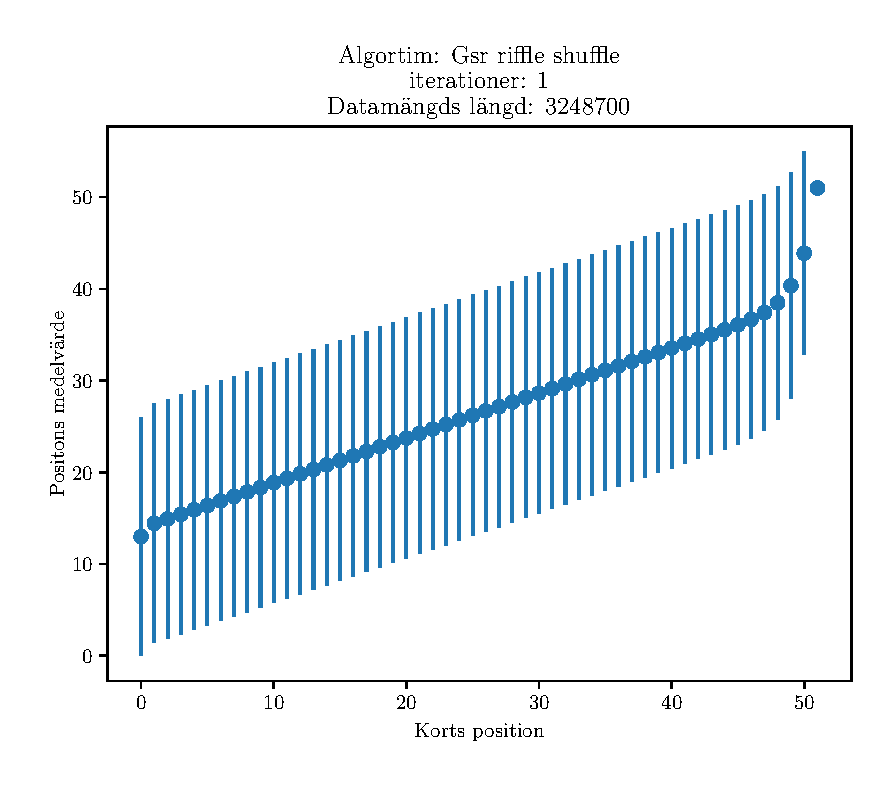
\includegraphics[width=0.8\textwidth, trim={0.8cm 0.8cm
	0.75cm 0.75cm}, clip]{gsr_riffle_shuffle-1}
	\captionsetup{width=0.5\textwidth}
	\caption{Resultatet från \gls{stdmean} testet  för \gls{gsr}
	Riffle Shuffle med \textbf{1} iteration.}
	\label{fig:gsr-1}
\end{figure}

\begin{figure}[H]
	\centering
	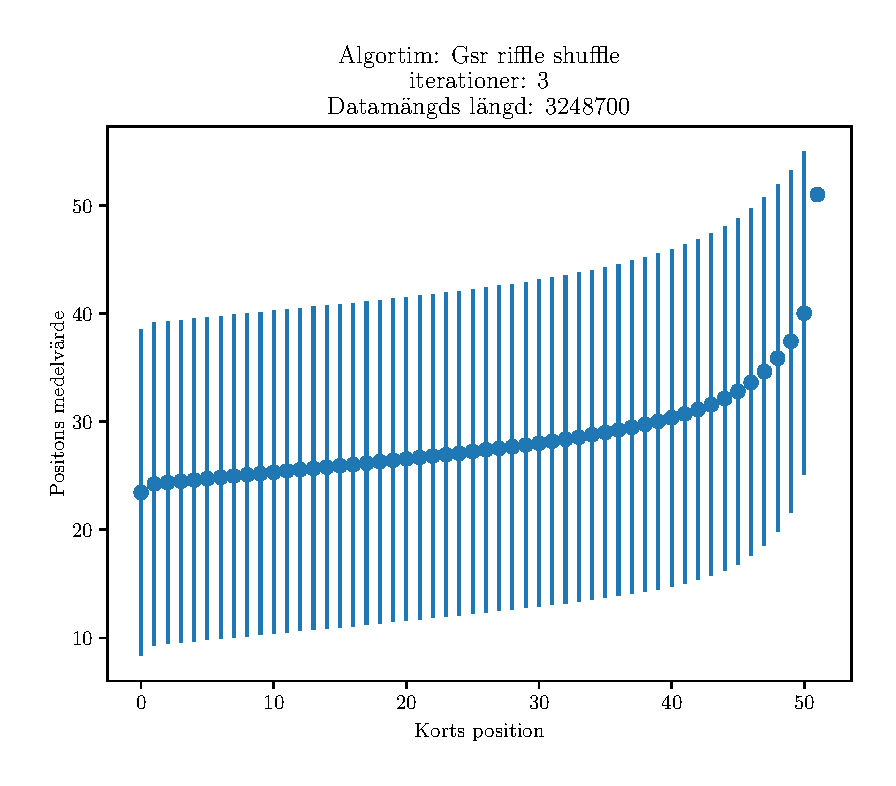
\includegraphics[width=0.8\textwidth, trim={0.8cm 0.8cm
	0.75cm 0.75cm}, clip]{gsr_riffle_shuffle-3} 
	\captionsetup{width=0.5\textwidth}
	\caption{Resultatet från \gls{stdmean} testet  för \gls{gsr}
	Riffle Shuffle med \textbf{3} iterationer.}
	\label{fig:gsr-3}
\end{figure}

\begin{figure}[H]
	\centering
	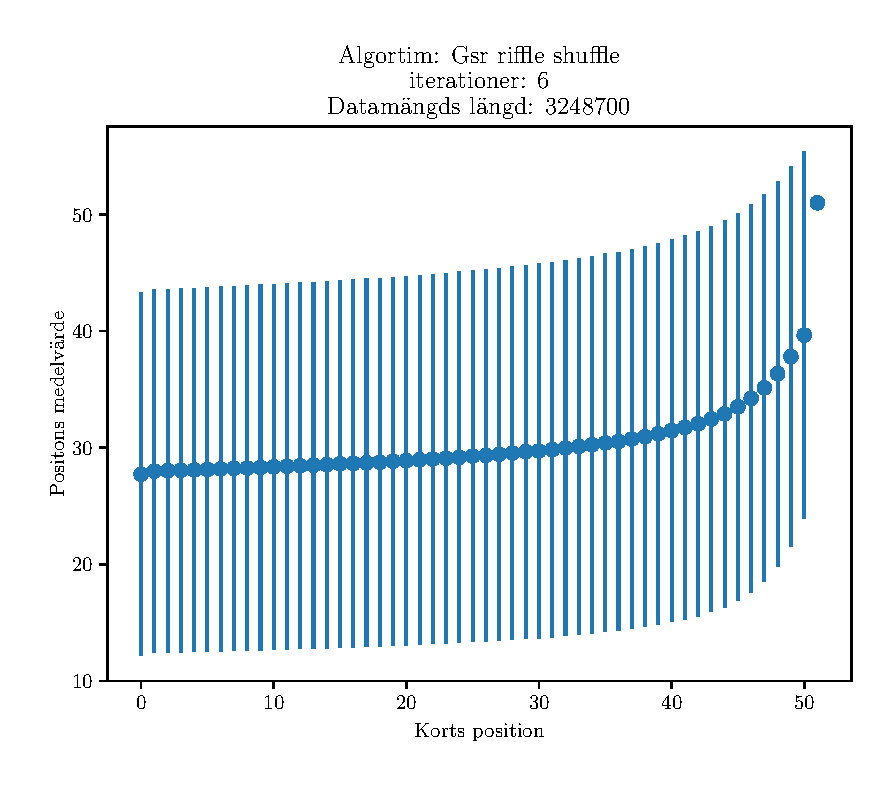
\includegraphics[width=0.8\textwidth, trim={0.8cm 0.8cm
	0.75cm 0.75cm}, clip]{gsr_riffle_shuffle-6} 
	\captionsetup{width=0.5\textwidth}
	\caption{Resultatet från \gls{stdmean} testet  för \gls{gsr} Riffle
	Shuffle med \textbf{6} iterationer.}
	\label{fig:gsr-6}
\end{figure}

\begin{figure}[H]
	\centering
	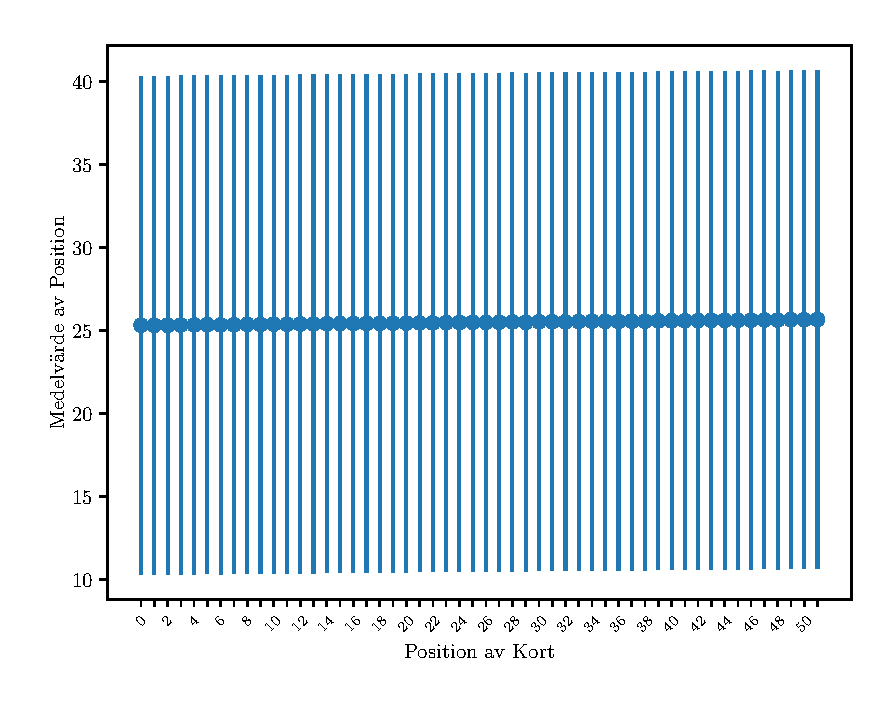
\includegraphics[width=0.8\textwidth, trim={0.8cm 0.8cm
	0.75cm 0.75cm}, clip]{gsr_riffle_shuffle-7} 
	\captionsetup{width=0.5\textwidth}
	\caption{Resultatet från \gls{stdmean} testet för \gls{gsr} Riffle Shuffle
	med \textbf{7} iterationer.}
	\label{fig:gsr-7}
\end{figure}

\begin{figure}[H]
	\centering
	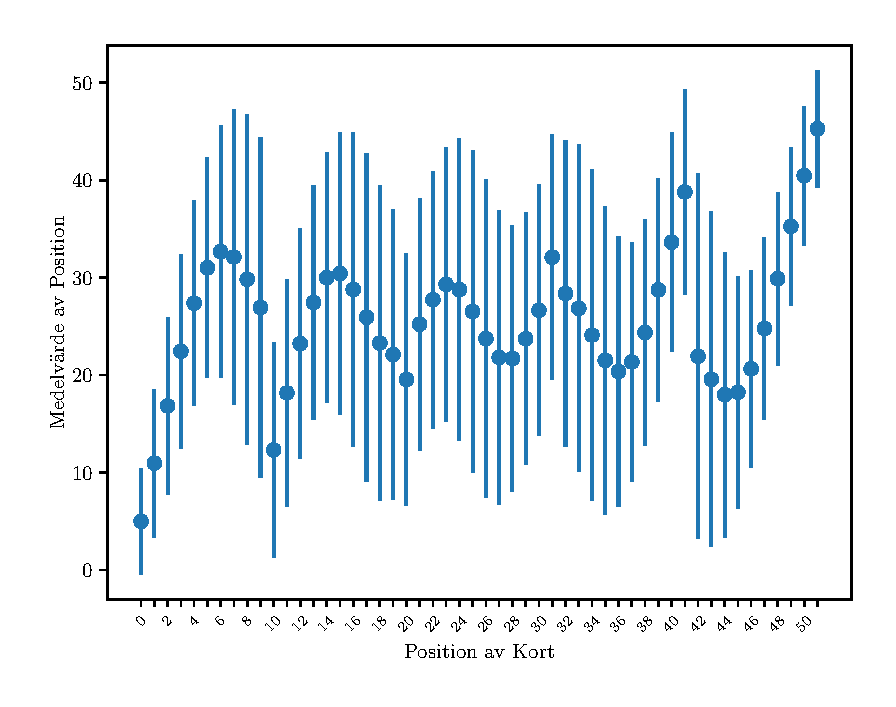
\includegraphics[width=0.8\textwidth, trim={0.8cm 0.8cm
	0.75cm 0.75cm}, clip]{six_pile_shuffle-1} 
	\captionsetup{width=0.5\textwidth}
	\caption{Resultatet från \gls{stdmean} testet för Six Pile
	Shuffle med \textbf{1} iterationer.}
	\label{fig:six-1}
\end{figure}

\begin{figure}[H]
	\centering
	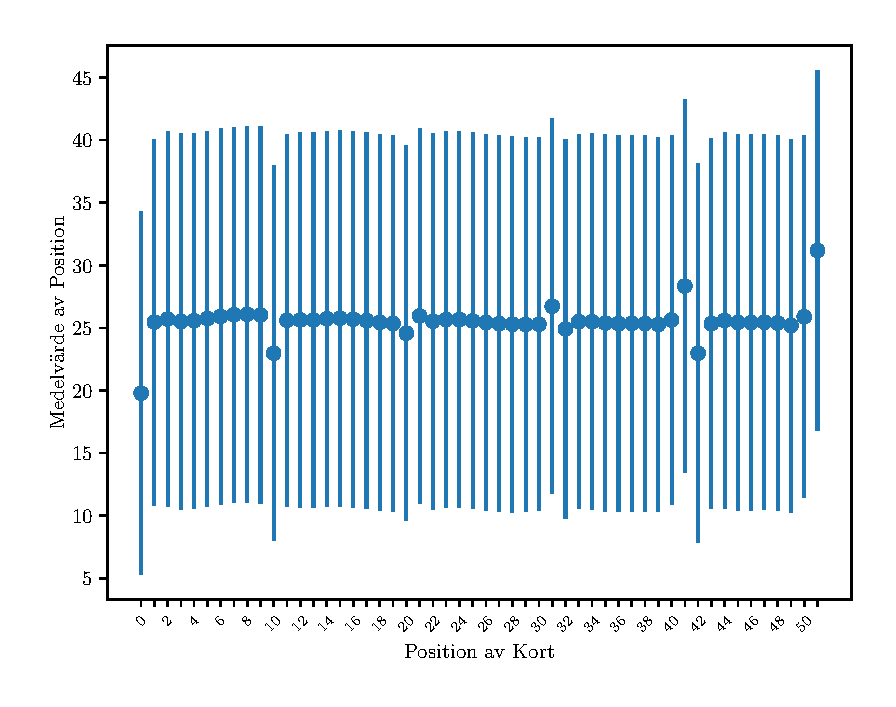
\includegraphics[width=0.8\textwidth, trim={0.8cm 0.8cm
	0.75cm 0.75cm}, clip]{six_pile_shuffle-2} 
	\captionsetup{width=0.5\textwidth}
	\caption{Resultatet från \gls{stdmean} testet för Six Pile
	Shuffle med \textbf{2} iterationer.}
	\label{fig:six-2}
\end{figure}

\begin{figure}[H]
	\centering
	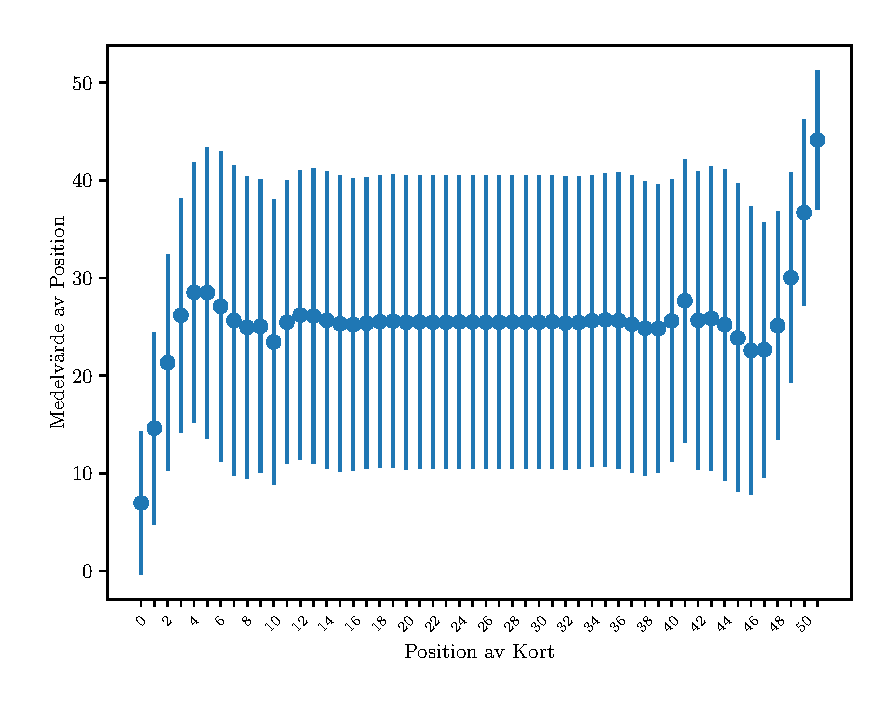
\includegraphics[width=0.8\textwidth, trim={0.8cm 0.8cm
	0.75cm 0.75cm}, clip]{soc_pile_shuffle-1} 
	\captionsetup{width=0.5\textwidth}
	\caption{Resultatet från \gls{stdmean} testet för \gls{soc} Pile
	Shuffle med \textbf{1} iteration.}
	\label{fig:soc-1}
\end{figure}

\begin{figure}[H]
	\centering
	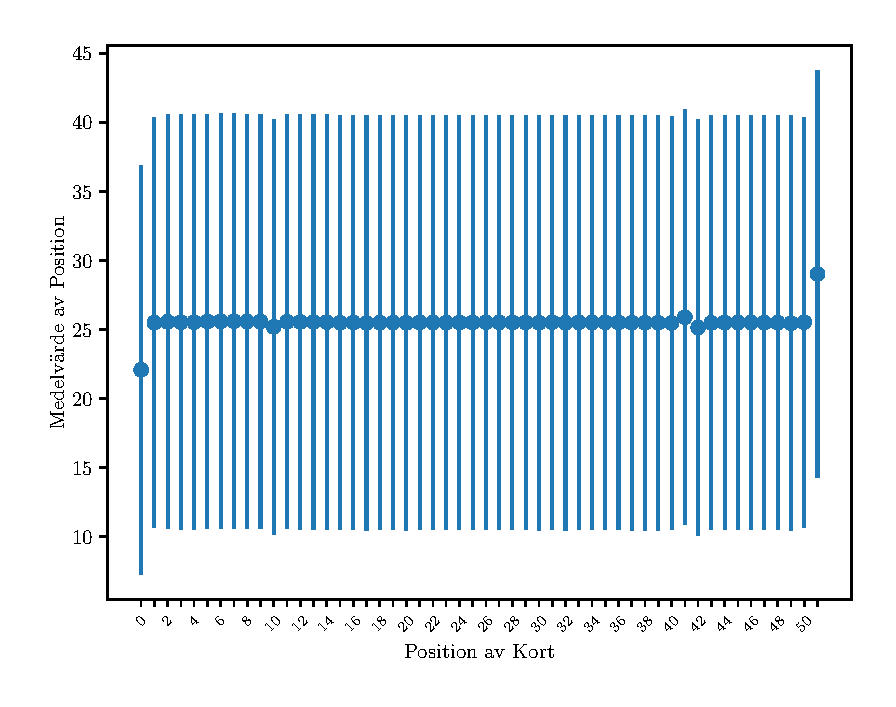
\includegraphics[width=0.8\textwidth, trim={0.8cm 0.8cm
	0.75cm 0.75cm}, clip]{soc_pile_shuffle-2} 
	\captionsetup{width=0.5\textwidth}
	\caption{Resultatet från \gls{stdmean} testet för \gls{soc} Pile
	Shuffle med \textbf{2} iterationer.}
	\label{fig:soc-2}
\end{figure}

\begin{figure}[H]
	\centering
	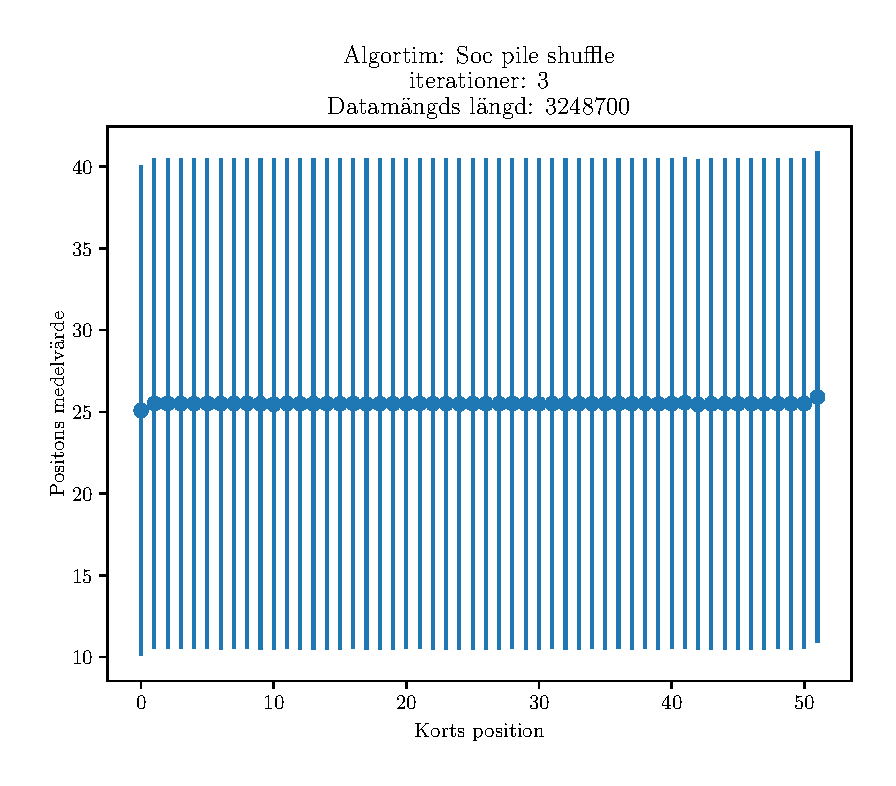
\includegraphics[width=0.8\textwidth, trim={0.8cm 0.8cm
	0.75cm 0.75cm}, clip]{soc_pile_shuffle-3} 
	\captionsetup{width=0.5\textwidth}
	\caption{Resultatet från \gls{stdmean} testet för \gls{soc} Pile
	Shuffle med \textbf{3} iterationer.}
	\label{fig:soc-3}
\end{figure}

\begin{figure}[H]
	\centering
	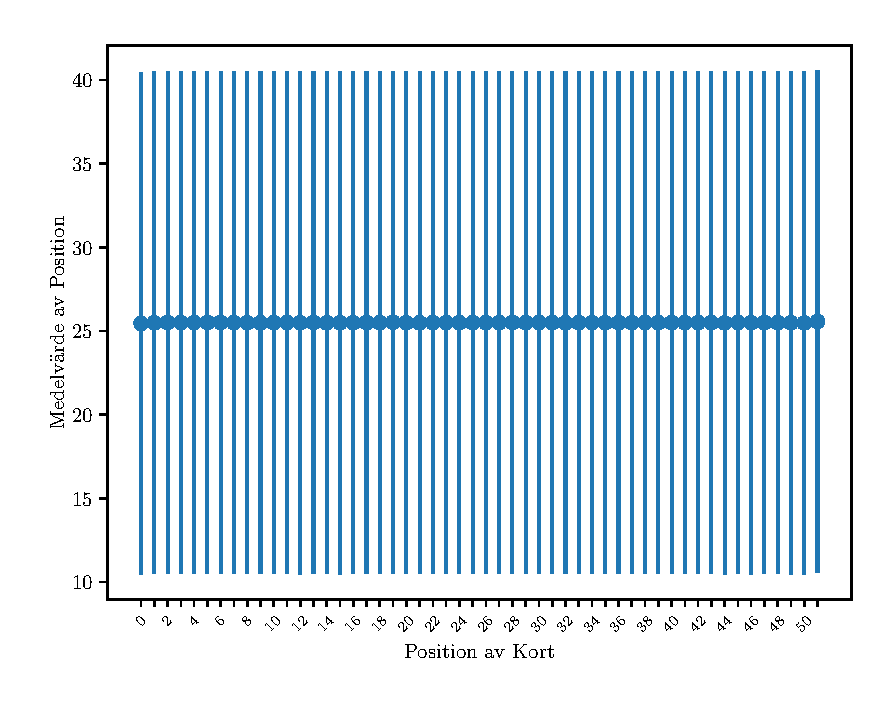
\includegraphics[width=0.8\textwidth, trim={0.8cm 0.8cm
	0.75cm 0.75cm}, clip]{soc_pile_shuffle-4} 
	\captionsetup{width=0.5\textwidth}
	\caption{Resultatet från \gls{stdmean} testet för \gls{soc} Pile
	Shuffle med \textbf{4} iterationer.}
	\label{fig:soc-4}
\end{figure}

\begin{figure}[H]
	\centering
	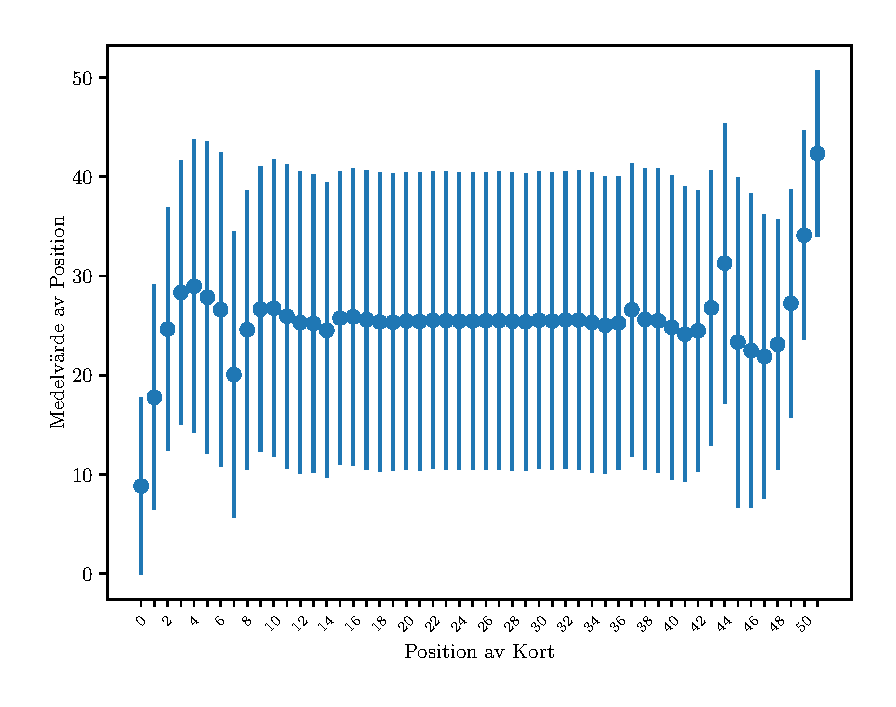
\includegraphics[width=0.8\textwidth, trim={0.8cm 0.8cm
	0.75cm 0.75cm}, clip]{ten_pile_shuffle-1} 
	\captionsetup{width=0.5\textwidth}
	\caption{Resultatet från \gls{stdmean} testet för Ten Pile
	Shuffle med \textbf{1} iteration.}
	\label{fig:ten-1}
\end{figure}

\begin{figure}[H]
	\centering
	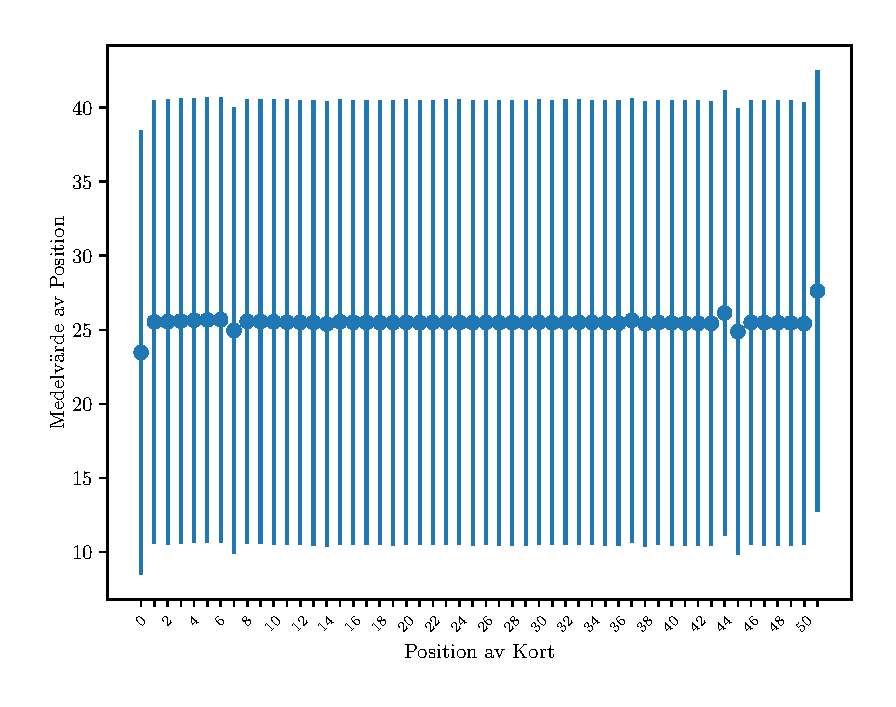
\includegraphics[width=0.8\textwidth, trim={0.8cm 0.8cm
	0.75cm 0.75cm}, clip]{ten_pile_shuffle-2} 
	\captionsetup{width=0.5\textwidth}
	\caption{Resultatet från \gls{stdmean} testet för Ten Pile
	Shuffle med \textbf{2} iterationer.}
	\label{fig:ten-2}
\end{figure}

\begin{figure}[H]
	\centering
	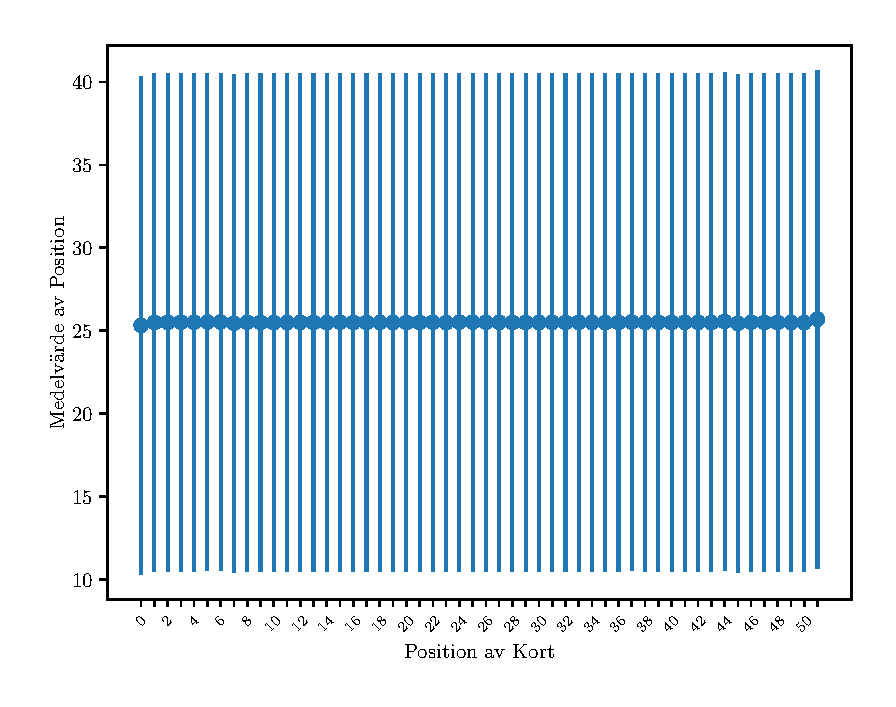
\includegraphics[width=0.8\textwidth, trim={0.8cm 0.8cm
	0.75cm 0.75cm}, clip]{ten_pile_shuffle-3} 
	\captionsetup{width=0.5\textwidth}
	\caption{Resultatet från \gls{stdmean} testet för Ten Pile
	Shuffle med \textbf{3} iterationer.}
	\label{fig:ten-3}
\end{figure}

\begin{figure}[H]
	\centering
	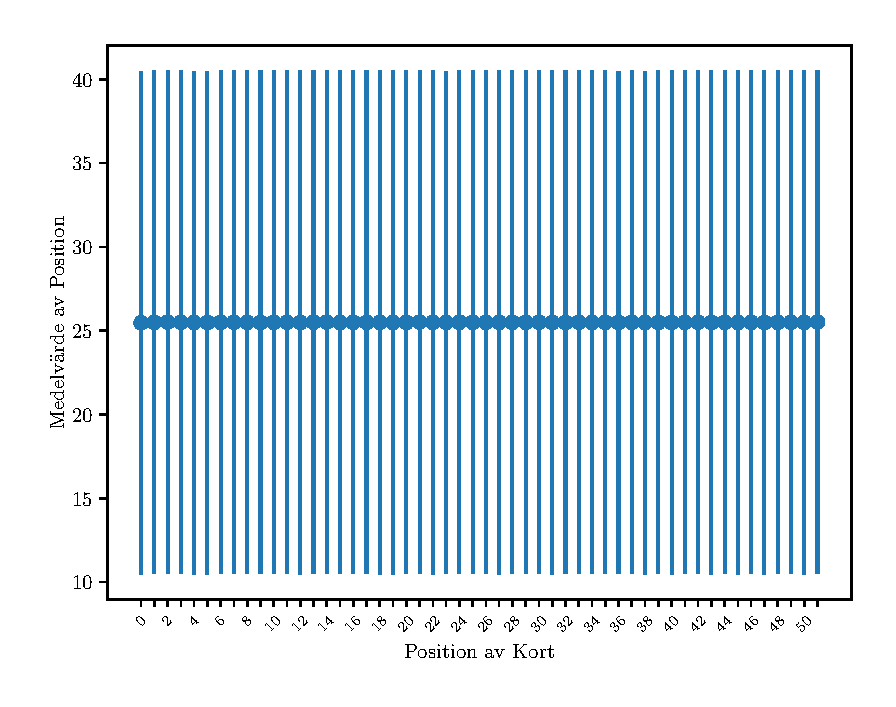
\includegraphics[width=0.8\textwidth, trim={0.8cm 0.8cm
	0.75cm 0.75cm}, clip]{ten_pile_shuffle-4} 
	\captionsetup{width=0.5\textwidth}
	\caption{Resultatet från \gls{stdmean} testet för Ten Pile
	Shuffle med \textbf{4} iterationer.}
	\label{fig:ten-4}
\end{figure}

\begin{figure}[H]
	\centering
	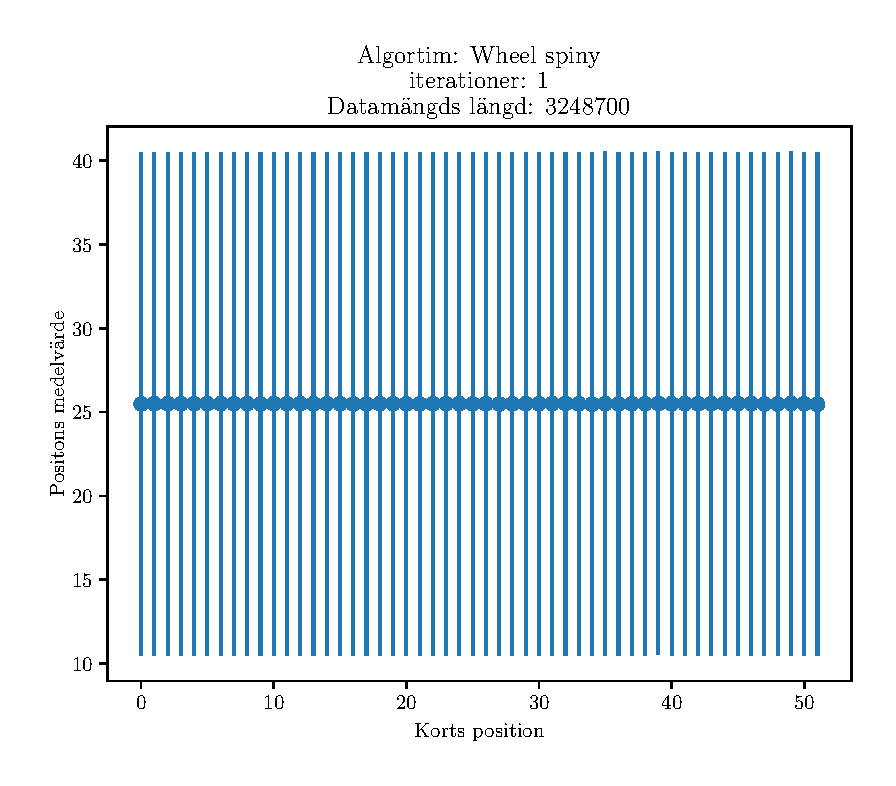
\includegraphics[width=0.8\textwidth, trim={0.8cm 0.8cm
	0.75cm 0.75cm}, clip]{wheel_spiny-1} 
	\captionsetup{width=0.5\textwidth}
	\caption{Resultatet från \gls{stdmean} testet för Wheel Fisher-Yates shuffle med \textbf{1} iteration.}
	\label{fig:wheel-1}
\end{figure}
